
\chapter{Introduction}


% \section{Contextualization}


    % [IA-GEN NA INDUSTRIA] 
    In the dynamic and ever-changing oil and gas (O\&G) industry,
    % \xexeo{eu acho que aqui falta alto. TEm um pouco há ver com o uso do "in the dynamic changing of the" não ser realmente muito adequado a "oil and gas industry", falta algo, um qualificador a mais (mercado? . Minha IA sugeriu mudar para "In the dynamic and ever-changing oil and gas (O\&G) industry", o que eu achei muito melhor}
    % \vitor{feito}
    \abbrev{O\&G}{oil and gas} 
    digital transformation has emerged as a key element to achieve operational efficiency, sustainability, and competitiveness. 
    At the forefront of this transformation are Large Language Models \abbrev{LLM}{Large Language Model}(LLM), which have the potential to process unstructured queries, map out alternatives, and advise users on possible actions \citep{Kar2023}. 
    We also note the advantage of increased engagement, cooperation, accessibility, and ultimately profitability. 
    These models redefine paradigms in knowledge management and information retrieval and impact a variety of other areas \citep{Eckroth2023}, making it crucial to adopt these technologies to remain competitive.    
    
    % [ESTUDO AUMENTO PRODUTIVIDADE] 
    A study conducted by \citet{Dellacqua2023}, in collaboration with the Boston Consulting Group, shows that in knowledge-intensive tasks, consultants equipped with access to LLMs such as GPT-4 not only completed tasks more efficiently (25.1\% more quickly on average) but also with substantially higher quality, achieving results more than 40\% better compared to those without AI assistance \citep{Dellacqua2023}.
    Increase in productivity of knowledge workers was 12\% on average.    
    A major oil company spent in 2023 \$2.8B with employee compensation \citep{Petrobras2024}.
    A potential increase of 12\% in knowledge workers productivity, given they represent 60\% of all employee, could represent \$204M annual savings in this scenario. 
    \xexeo{Aqui está um problema clássico. Você quer fornecer um dado mas provavelmente não quer dizer que é a Petrobras. Mas provavelmente esse dado está em algum relatório público. Não consegue ele de algum lugar e aí pode citar?} 
    \vitor{feito}   
    
    % [AUMENTO DO PIB DEVIDO A GEN AI] 
    Broader economic indicators predict significant transformations due to generative AI (Gen-AI) across various industries.
    A report from Goldman Sachs \citep{Hatzius2023} highlights that Gen-AI is poised to increase global GDP by nearly 7\%, increasing productivity growth by 1.5 percentage points over the next decade. 
    This economic uplift is expected due to AI's ability to automate complex workflows and create new business opportunities, significantly impacting employment and productivity sectors worldwide.


            
    % [PROBLEMA DE DADOS NA INDUSTRIA EM GERAL] 
    Expanding on the broader discussion on data utilization within organizations, an important issue is the challenge of extracting relevant information from extensive databases \citep{Singh2023}. 
    Initially, the challenge of knowing, finding, and accessing data poses a significant obstacle to decision-making processes. 
    Collaborators at O\&G companies often face the intensive task of manually searching large data repositories to find useful information.


    
    % [PROBLEMA DE DADOS NO O\&G] 
    Focusing specifically on the activities of drilling and completion of offshore and onshore wells, a major challenge lies in the inherently complex and technical nature of the data involved, which can be from various types: operations, projects, technologies, supply chains, and others. 
    Inefficiency in leveraging large volumes of unstructured data worsens these challenges, as observed by \citet{Singh2023}. 
    A significant amount of the data generated and collected in this sector is unstructured, ranging from text reports and emails to images and videos of exploration and production activities. 
    Examples include hundreds of daily operational reports from drilling rigs, well execution projects, nonproductive time (NPT) reports, and operational lessons learned documents, as illustrated in Figure \ref{fig:report_example}. 
    As a result, valuable information can remain untapped, and the potential to find insights, informed decision-making, and innovation is significantly compromised.
    \citet{Singh2023} showcases the capabilities and potential of Generative AI-enabled chatbots for the O\&G sector, particularly in enhancing drilling and production analytics to achieve better business results. The author concludes that companies that adopt these technologies in the coming years will see clear advantages.     
    
    \begin{figure}[t]
        \centering
        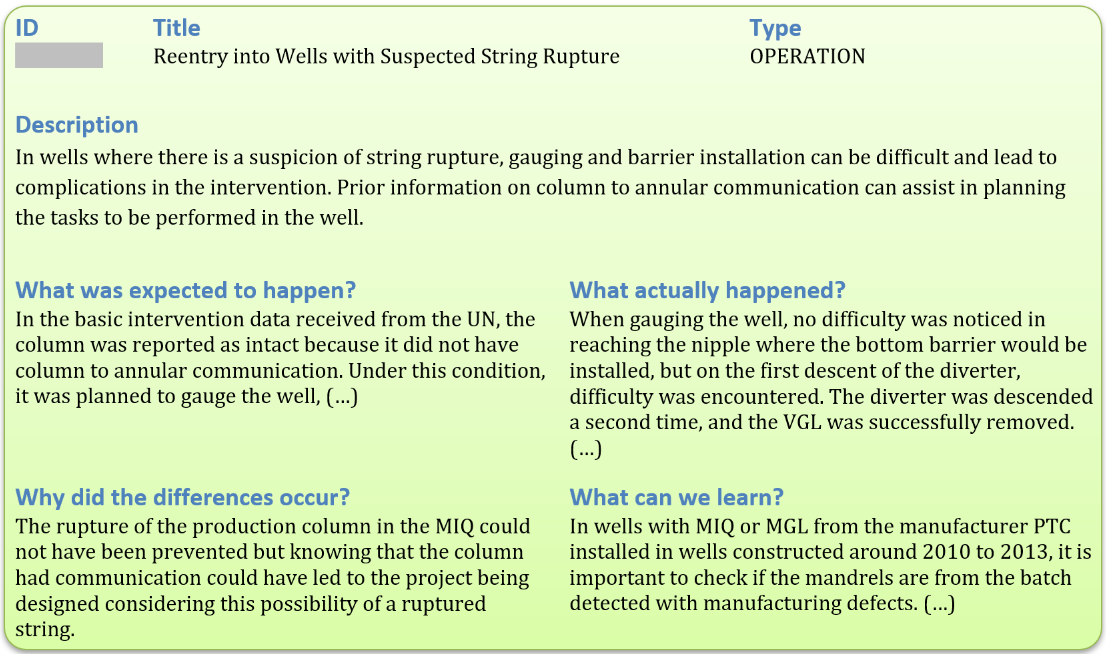
\includegraphics[width=1\textwidth]{images/report_example.png}
        \caption{Sample of drilling \& completion learned lesson partial document. (translated from Portuguese)}
        \label{fig:report_example}
    \end{figure}           
    
    However, the deployment of such technologies presents limitations and introduces challenges, including biased data, hallucinations, lack of explainability, and logical reasoning errors, among others \citep{Hadi2023}, which require a balanced approach to harness their potential in a responsible manner.    
    Although previous research has focused mainly on the broader applications of AI in industry, the novelty of our research lies in its original examination of the specific challenges and solutions presented by the complex, technical and unstructured data inherent in O\&G operations. 
    By comparing single- and multi-agent systems, this study fills a knowledge gap, providing empirical insights into the effectiveness of different Gen-AI architectures in a domain where such studies are scarce. 
    
    The adoption of these technologies by a major oil company underscores their potential to revolutionize data analysis and management, presenting an opportunity for deeper exploration and application.

\section{Business Scope Delimitation}

    To contextualize the scope of this study, it is necessary to understand the life cycle of an oil field, which begins with Exploration and progresses to the Development of Production, followed by effective production, and culminates in decommissioning \citep{Badiru2016}. Gen-AI has the potential to impact each of these phases, but the focus of this work lies in the operations of the development and maintenance stages.
            
    Well construction is a highly specialized activity that involves drilling and completion of wells for hydrocarbon extraction \citep{Thomas2004}. In this context, Gen-AI can be applied in various ways. 
    For example, a chatbot could manage knowledge by answering queries about operations and well projects by retrieving information from the organization's databases. 
    Additionally, LLM-based agents could be used in executive project review to ensure that drilling or completion operations comply with the organization's standards and adhere to best operational practices. 
    Moreover, Gen-AI could perform inference in unstructured databases to extract specific information from text reports and obtain structured data. This business scope emphasizes the importance of Gen-AI in the construction and maintenance of wells.

    \subsection{Key Information Sources in Well Engineering} \label{sec:information-sources}

        To fully appreciate the challenges in this domain, it is important to understand the primary data sources that specialists interact with daily. The following sources, used in this research's experiments, exemplify the complex information landscape of well engineering:

        \paragraph{Operational Learned Lessons} During drilling, completion, and workover interventions, documents called Knowledge Items are written by specialists, as depicted in Fig~\ref{fig:report_example}. These can be of four types: Technical Alert, Learned Lesson, Good Practice, and Well Observation. This system serves as a critical tool for knowledge management, considering the large number and variety of specialists involved and well operations performed.

        \paragraph{Operational NPTs (Non-Productive Time)} This data source contains structured records of anomalies that occurred during well interventions, detailing the title, description, location, operation type, responsible sector, rig involved, time lost, and event dates. These data are critical for the industry, as NPTs represent periods when operations are interrupted. The identification and analysis of these events are essential for continuous process improvement, cost reduction, and increased operational efficiency.

        \paragraph{Collaborator Finder} The third data source is a collaborator finder, an important internal tool for consulting and managing employee data. This system allows for the quick identification of employees through information such as name, workplace, and role. The importance of this tool lies in the ability to cross-reference employee data with operational events, enabling a more complete analysis by an intelligent agent.

\section{Objectives}

    % This research directly addresses the challenges facing major oil companies. 
    % By investigating the comparative advantages and limitations of various Gen-AI architectures, including single and multi-agent systems, for Q\&A and Text-to-SQL tasks, this study aims to identify the most efficient and cost-effective solutions.
    
    % The specific objectives of this research are to assess the suitability and effectiveness of multi-agent systems based on LLMs for complex, domain-specific tasks in well engineering, aiming to streamline information access and decision-making.
    
    % The study will compare single-agent and multi-agent AI systems in terms of their ability to address well engineering queries. Finally, it will map the potential obstacles and limitations associated with deploying Gen-AI applications.
            
    % The insights gained from this research will directly contribute to O\&G companies strategic goals by improving access to well engineering information and automated data analysis tasks. 
    % A comprehensive understanding of the challenges and limitations associated with Gen-AI will enable informed decisions about its adoption, maximizing the return on investment. 

    The primary goal of this dissertation is to systematically evaluate and compare the effectiveness, efficiency, and practical viability of different LLM-based architectures for resolving domain-specific information retrieval challenges in well construction engineering. 
    This research aims to move beyond generalized performance metrics to provide specific, empirical insights into how architectural choices impact outcomes in a industrial setting.

    To achieve this overarching goal, the following specific objectives have been defined:

    \begin{enumerate}
        \item \textbf{Design and Implement LLM Artifacts:} To design and implement a set of distinct RAG architectures, including non-agentic (baseline and router-based) and agentic (single-agent and multi-agent) systems, tailored to the operational context of well construction.

        \item \textbf{Evaluate Performance Quantitatively:} To evaluate the performance of these artifacts on domain-specific tasks using both expert-led qualitative assessments and automated quantitative metrics, including truthfulness, precision, recall, and F1-score.

        \item \textbf{Analyze Cost-Effectiveness:} To conduct a comparative analysis of the economic efficiency of each architecture, focusing on the trade-offs between performance gains and the computational costs associated with LLM API usage.

        \item \textbf{Derive Actionable Guidance:} To identify the key challenges, limitations, and failure modes of each architecture within a specialized technical domain, and to derive practical, evidence-based guidelines for the strategic adoption of these technologies in the oil and gas industry.
    \end{enumerate}

    % To achieve these objectives, this research was conducted through two distinct experimental phases. The first, carried out in 2024, focused on a foundational comparison between single and multi-agent architectures, which revealed that, although the multi-agent architecture achieved 28\% higher truthfulness in Q\&A tasks, its cost was on average 3.7 times higher. Furthermore, the single-agent architecture proved to be surprisingly more effective in Text-to-SQL tasks. 
    
    % The rapid evolution of generative AI frameworks and models prompted a second, more advanced experiment in 2025. This second phase built upon the initial findings, also employing non-agentic workflows as baseline and a more rigorous, quantitative evaluation methodology to address the challenges identified in the first experiment and automated evaluation based on the concept commonly reffered to as "LLM-as-judge" (\citep{Gu2025}).
    
    \xexeo{Acho que pode aumentar um pouco isso, já falar dos resultados (dissertação tem spoiler), motivar o segundo a partir dos resutlados do primeiro e botar depois das questões de pesquisa (leia o todo), sempre alinhando tudo (questão de pesquisa - experimento - conclusões}
    \vitor{Incluído spoiler e ponte do 1o justificando o 2o experimento.}

    <<<<PENDENTE>>>>

    FAZER ALINHAMENTO FINAL (QUESTÃO DE PESQUISA - EXPERIMENTO - CONCLUSÕES)
    
    DETALHAMENTO LLM: "BOTAR DEPOIS DAS QUESTÕES DE PESQUISA" E "SEMPRE ALINHANDO TUDO"
    ESTA É A "LINHA DE OURO" (GOLDEN THREAD) DE UMA DISSERTAÇÃO. TUDO PRECISA ESTAR CONECTADO. A ESTRUTURA QUE ELE SUGERE CRIA UM FLUXO MUITO LÓGICO PARA O LEITOR:
    
    OBJETIVOS: O QUE VOCÊ QUER ALCANÇAR (VISÃO GERAL).
    
    QUESTÕES DE PESQUISA (A SEREM ADICIONADAS): AS PERGUNTAS ESPECÍFICAS E FOCADAS QUE SUA PESQUISA VAI RESPONDER.
    
    PARÁGRAFO COM "SPOILER" (O QUE ESTAMOS DISCUTINDO): UM RESUMO DE COMO VOCÊ RESPONDEU A ESSAS PERGUNTAS E O QUE ENCONTROU.
    
    CONCLUSÕES (NO FINAL DA DISSERTAÇÃO): ONDE VOCÊ RESPONDE FORMALMENTE ÀS QUESTÕES DE PESQUISA, USANDO OS RESULTADOS DETALHADOS DOS EXPERIMENTOS.

    AO COLOCAR O PARÁGRAFO DE "SPOILER" DEPOIS DAS QUESTÕES DE PESQUISA, VOCÊ CRIA UMA CONEXÃO DIRETA: "PARA RESPONDER A ESTAS PERGUNTAS (QUESTÃO 1, QUESTÃO 2...), EU CONDUZI ESTES EXPERIMENTOS (EXPERIMENTO 1, EXPERIMENTO 2), QUE ME LEVARAM A ESTAS DESCOBERTAS PRINCIPAIS (RESULTADO A, RESULTADO B)."

    ESSA ESTRUTURA AMARRA TODA A SUA DISSERTAÇÃO, TORNANDO-A COESA, LÓGICA E FÁCIL DE ACOMPANHAR.
    <<<<FIM>>>>

    \todo[inline]{Ok, está bom, porém seria melhor para dissertação se agora você definisse questões de pesquisa. Essas questões de pesquisa serão respondidas na conclusão, a partir do que você fez. Eu só li até aqui, então não tenho sugestões fortes agora, mas as questões podem ser coisas coisa: Qual a eficácia e eficiência de LLMs para extrair dados de bases .... Como sistemas single e multi agentes se comparam... Elas podem ser bem melhores e bem mais objetivas e ao longo do texto, se eu detectar alguma , escrevo. A questão é perguntar aqui no fim da introdução e responder na conclusão, caracterizando a colaboração
    \newline \newline SERÁ FEITO NO FIM}


% \todo[inline]{\textbf{VITOR: CONCLUÍDO} \newline \newline 
%     Ok, faltou a metodologia e tem que ter. Tem que explicar a metodologia genérica de sua pesquisa. Eu agora não sei bem o que se ajeita, mas vejo que talvez possa descrever como DSR ou outro método que implique em ações reais em um local. É importante notar que você descreve uma metodologia nos seus experimentos que é um processo de pesquisa (e isso não está errado), porém aqui há deve ser usado um conceito de metodologia mais amplo, ligado a epistemologia. Argumentos em função da DSR: Design Science Research (DSR) [sim, pedi para o ChatGPT, mas eu já meio que concordava]
%     A Design Science Research é a classificação mais apropriada para a metodologia empregada, pelos seguintes motivos:
%     \textbf{Artefato proposto}: A pesquisa visa comparar e melhorar arquiteturas de sistemas baseadas em LLMs aplicadas a tarefas específicas de engenharia de poços, o que se alinha à criação e avaliação de artefatos — elemento central da DSR.
%     \textbf{Avaliação empírica}: Foram realizados dois ciclos de experimentos com diferentes configurações de agente único e multiagente, com dados reais da indústria de O\&G e validação por especialistas.
%     \textbf{Ciclos iterativos}: O segundo experimento se baseia explicitamente nos resultados do primeiro, sugerindo um processo iterativo de refinamento de artefatos — outro elemento típico de DSR.
%     \textbf{Relevância prática + rigor científico}: O trabalho visa resolver um problema concreto de empresas do setor de petróleo e gás, mas com critérios e métricas de avaliação quantitativas rigorosas.
%     \textbf{Conclusão}: Mesmo sem ter sido explicitamente rotulada como DSR na dissertação, a estrutura e objetivos da pesquisa indicam fortemente que ela segue os princípios dessa metodologia.
%     \newline \newline \textbf{VITOR: CONCLUÍDO}}


\section{Research Questions}

    To guide this investigation and structure the research, the study addresses a central research question, which is broken down into three specific sub-questions. These questions will be formally answered in the conclusion, based on the evidence gathered from the two experimental cycles.

    \vspace{\baselineskip}
    \begin{tcolorbox}[colback=gray!10, colframe=gray!40, title=\textbf{Main Research Question}]
    How do different LLM based architectures, ranging from non-agentic Retrieval-Augmented Generation (RAG) pipelines to multi-agent systems, compare in terms of performance, efficiency, and practical viability when applied to domain-specific information retrieval tasks in well construction engineering?
    \end{tcolorbox}
    \vspace{\baselineskip}

    \paragraph{RQ1: Performance and Task-Dependency} Which architecture (non-agentic, single-agent, or multi-agent) provides the highest factual accuracy and overall performance for different types of domain-specific tasks, specifically complex Question-Answering (Q\&A) and structured Text-to-SQL generation?

    \paragraph{RQ2: Cost-Effectiveness} What is the relationship between architectural complexity and economic cost? How do the performance benefits of more complex systems (e.g., multi-agent) weigh against their significantly increased computational (API) costs, and what are the implications for practical deployment?

    \paragraph{RQ3: Agentic Systems and Domain Specificity} Under what conditions do agentic architectures, with their capacity for cyclical reasoning and reflection, offer a tangible performance advantage over simpler, non-agentic RAG workflows in a highly specialized technical domain where the LLM has a significant "knowledge deficit"?

    \vspace{\baselineskip}

    To answer these questions, this research was conducted through two distinct experimental cycles. The first, carried out in 2024, established a foundational comparison, revealing that while a multi-agent architecture achieved 28\% higher truthfulness in Q\&A tasks, its cost was on average 3.7 times higher. Furthermore, a single-agent architecture proved to be surprisingly more effective in Text-to-SQL tasks.

    The rapid evolution of generative AI frameworks and models prompted a second, more advanced experiment in 2025. This second phase built upon the initial findings, employing non-agentic workflows as a baseline and a more rigorous, automated evaluation methodology based on the "LLM-as-judge" concept \citep{Gu2025}. This led to a crucial and counter-intuitive discovery: a non-agentic architecture using an intelligent router to select the correct knowledge source decisively outperformed both single and multi-agent systems. This finding suggests that in specialized domains where the LLM lacks deep pre-trained knowledge, the reflective capabilities of agentic systems are less effective than a streamlined, well-directed retrieval process, fundamentally shaping the answers to our research questions.



\section{Research Methodology}
  
    This research follows the Design Science Research (DSR) methodology, a framework particularly suited for studies that develop and evaluate technological artifacts to address specific organizational problems. DSR provides a structured approach for creating innovative solutions while maintaining scientific rigor through empirical validation \citep{hevner2007three}.
    
    \begin{figure}[h]
    \centering
    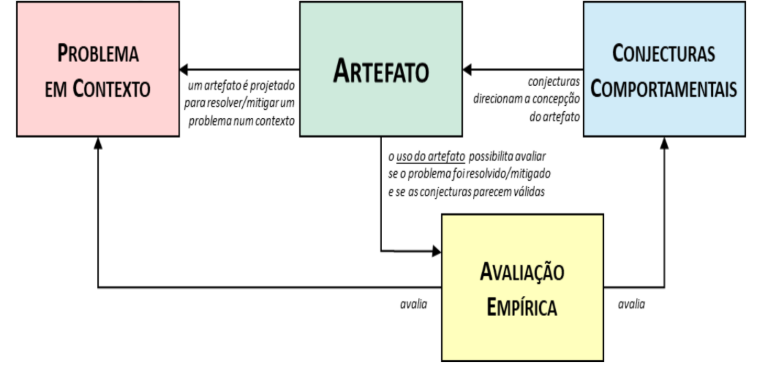
\includegraphics[width=0.8\textwidth]{images/dsr-model.png}
    \caption{Main elements of DSR-Model, translated from \citet{Oswald2023}.}
    \label{fig:dsr-model}
    \end{figure}
    
    \subsection{Design Science Research Framework}
    
        The DSR methodology employed in this study consists of four interconnected elements, as illustrated in Figure~\ref{fig:dsr-model}:
        
        \begin{enumerate}
        \item \textbf{Problem in Context}: Identifying and defining a relevant organizational challenge within its specific environment
        \item \textbf{Artifact}: Designing and developing a technological solution to address the identified problem
        \item \textbf{Behavioral Conjectures}: Formulating hypotheses about how the artifact will function and impact the problem space
        \item \textbf{Empirical Evaluation}: Systematically testing the artifact to validate its effectiveness and the underlying conjectures
        \end{enumerate}
        
        This cyclical framework guides both the research design and execution, ensuring that the developed artifacts are not only technically sound but also practically relevant.
    
    \subsection{Application of DSR in This Research} \label{sec:dsr-application}
        
        \subsubsection{Problem in Context}
        
        This study addresses the challenge of efficiently extracting relevant information from extensive technical databases in the oil and gas industry, specifically in well construction and maintenance operations. 
        
        \begin{table}[h]
            \centering
            \caption{Characteristics of the Problem Context}
            \begin{tabular}{|p{0.45\textwidth}|p{0.45\textwidth}|}
            \hline
            \textbf{Challenge Aspect} & \textbf{Description} \\
            \hline
            Data Structure & Large volumes of unstructured data (operational reports, lessons learned documents, NPT reports) \\
            \hline
            Technical Complexity & Domain-specific terminology and complex relationships \\
            \hline
            Business Impact & Significant potential economic impact from improved knowledge access \\
            \hline
            \end{tabular}
            \label{tab:problem-context}
        \end{table}
        
        \subsubsection{Artifacts}
        
        Two primary artifacts were designed and implemented, illustrated in Figure~\ref{fig:artifacts}, using state-of-the-art language models (GPT-3.5-turbo and GPT-4) and integrated with domain-specific knowledge bases through various retrieval mechanisms.
        
        \begin{figure}[h]
        \centering
        \begin{minipage}{0.45\textwidth}
            \centering
            \fbox{\begin{tabular}{c}
            \textbf{Single-Agent LLM System} \\
            \small A centralized architecture where one \\
            \small language model agent handles the entire \\
            \small question-answering process with \\
            \small access to multiple tools
            \end{tabular}}
        \end{minipage}
        \hfill
        \begin{minipage}{0.45\textwidth}
            \centering
            \fbox{\begin{tabular}{c}
            \textbf{Multi-Agent LLM System} \\
            \small A collaborative architecture where \\
            \small multiple specialized agents work together \\
            \small under coordination to process queries \\
            \small  
            \end{tabular}}
        \end{minipage}
        \caption{Primary Artifacts Developed in This Research}
        \label{fig:artifacts}
        \end{figure}
        
        
        \subsubsection{Behavioral Conjectures}
        
        The research was guided by several key conjectures:
        
        \begin{tcolorbox}[colback=gray!10, colframe=gray!40, title=Key Research Conjectures]
            \begin{itemize}
            \item Multi-agent systems will demonstrate higher accuracy in complex technical queries due to their ability to distribute cognitive load and specialize in different aspects of the problem
            \item The performance advantages of multi-agent systems will vary by task type (Q\&A vs. Text-to-SQL)
            \item More advanced language models will yield better performance but at significantly higher LLM financial costs
            \item The economic efficiency (performance-to-cost ratio) will be a critical factor in determining practical implementation viability
            \end{itemize}
        \end{tcolorbox}
        
        \subsubsection{Empirical Evaluation}
        
        The evaluation was conducted through two distinct experimental phases (summarized in Table~\ref{tab:experiments}), allowing for iterative refinement of both the artifacts and the evaluation methodology, addressing limitations identified in the first experiment while adapting to the rapid evolution of language model capabilities.
        
        \begin{table}[h]
        \centering
        \caption{Comparison of Experimental Phases}
        \begin{tabular}{|p{0.15\textwidth}|p{0.38\textwidth}|p{0.38\textwidth}|}
        \hline
        \textbf{Aspect} & \textbf{First Experiment (2024)} & \textbf{Second Experiment (2025)} \\
        \hline
        Focus & Comparative analysis of single and multi-agent architectures & Extended evaluation incorporating non-agentic workflows as baseline \\
        \hline
        Evaluation Methods & Expert validation by domain specialists & Automated assessment using "LLM-as-judge" approach \\
        \hline
        Metrics & Truthfulness, performance, and LLM cost & Precision, recall, and F1-score \\
        \hline
        Outcomes & Identification of key challenges and limitations & More rigorous quantitative evaluation methodology \\
        \hline
        \end{tabular}
        \label{tab:experiments}
        \end{table}

    
    % \subsection{Research Quality and Validity}
    
    %     To ensure research quality and validity, several measures were implemented, as shown in Figure~\ref{fig:research-quality}. 
    %     By adhering to the DSR methodology, this research maintains a balance between practical utility and scientific rigor, producing artifacts that address real organizational needs while contributing to the theoretical understanding of multi-agent LLM systems in specialized technical domains.
        
    %     \begin{figure}[h]
    %         \centering
    %         \begin{tikzpicture}
    %         \node[draw, rounded corners, fill=blue!10, text width=0.3\textwidth, align=center] (a) at (0,0) {\textbf{Triangulation}\\\small Using multiple data sources, evaluation methods, and expert perspectives};
    %         \node[draw, rounded corners, fill=blue!10, text width=0.3\textwidth, align=center] (b) at (6,0) {\textbf{Reproducibility}\\\small Detailed documentation of experimental procedures, prompts, and configurations};
    %         \node[draw, rounded corners, fill=blue!10, text width=0.3\textwidth, align=center] (c) at (0,-4) {\textbf{Practical Relevance}\\\small Direct application to real-world operational challenges};
    %         \node[draw, rounded corners, fill=blue!10, text width=0.3\textwidth, align=center] (d) at (6,-4) {\textbf{Theoretical Contribution}\\\small Insights into comparative advantages of different agent architectures};
    %         \draw[->] (a) -- (b);
    %         \draw[->] (b) -- (d);
    %         \draw[->] (a) -- (c);
    %         \draw[->] (c) -- (d);
    %         \end{tikzpicture}
    %         \caption{Research Quality Assurance Framework}
    %         \label{fig:research-quality}
    %     \end{figure}
        
        

\section{Thesis Structure}



    ****SERÁ FEITO POR ÚLTIMO****
